\documentclass[11pt]{article}
\usepackage[top=1.00in, bottom=1.0in, left=1.1in, right=1.1in]{geometry}
\renewcommand{\baselinestretch}{1}
\usepackage{graphicx}
\usepackage{natbib}
\usepackage{amsmath}
\usepackage{hyperref}
\usepackage{todonotes}

\def\labelitemi{--}


\begin{document}
\bibliographystyle{/Users/Lizzie/Documents/EndnoteRelated/Bibtex/styles/besjournals}
\renewcommand{\refname}{\CHead{}}

\title{Effects of phenology on plant community assembly and structure }
\author{Elsa E. Cleland \& E. M. Wolkovich}
\date{\today}
\maketitle
\tableofcontents

\setlength{\parindent}{0cm}
\setlength{\parskip}{5pt}

% Note to Lizzie: Check for TODO notes throughout. 

\section{Main text}


\emph{Definition to fit in ...} 
% timing of recurring growth and reproductive events (Ackerly)
% Isabelle is more of the `timing of recurring life history events ilk' and she stressed the seasonality of phenology as needing to be in the definition, but then we discussed tropical phenology etc. and she came around to this.
We define phenology as the timing of critical stages of growth and reproduction and the transitions between them. This definition is intentionally more inclusive than some other definitions, which focus on recurring or seasonal events, and thus can narrow phenology to only certain plant types or biomes (e.g., woody species in the temperate zone). This artificial narrowing to us can preclude understanding the selective pressures on phenology that---as we outline below---are critical for understanding the role of phenology in community assembly. Our definition thus includes both tree leafout, and seed germination of annual plants at the same time in encompasses fruiting, flowering and importation transitions in and out of these phases, such as dormancy and vernalization.

Phenological `events' are rarely one moment in time ... get into distributions and plasticity here? Or leave it where I have it below?

\subsection*{Phenological assembly: From the abiotic to biotic environments}
% Section 2
% TODO: Need ref for Janneke 2012 review (HilleRisLambers et al.)
Communities assemble from a regional species pool through a series of abiotic and biotic sorting processes. At the largest scale, a community's assemblage is limited by species in the larger regional pool---species well suited to an environment may thus not appear in it unless they are present in the this regional pool. From this pool, species are filtered based on the abiotic environmental conditions of a particular location---species must be able to persist through an environments extremes in hot, cold, dry, wet and other factors to pass through this `environmental filtering' step of assembly. This collection of potential species that could form a community is then filtered once more---by the pool of species itself. 

Competitive, facilitative, predatory and all other biotic interactions determine which species together can co-occur in the long term. If two species compete too strongly, then only the stronger competitor will remain in the community at this step, and similarly obligate mutualists, predators and parasites will persist only if the other species they require are present in the community. This final stage of assembly is where much of community ecology has focused over its history as a subdiscipline, driving theories of coexistence, including whether species even truly `coexist' or merely are on a slow walk to extinction for all but one species in each community \citep{Hubbell:2001vo}. 

Phenology enters community assembly at both the environmental and biotic filtering steps. Species phenologies must match the environment to pass the first filter: their growth and reproduction must be timed to match periods when the environment is mild and resource-rich enough for these events. Thus, in an environment with cold sub-freezing winters, species generally must have well-timed dormancy to avoid leafing out in the middle of the winter when they would loose all new tissue. Similarly, arid and tropical environments impose filters against certain phenologies. Once a set of species pass the environmental filter, phenology matters again at the biotic filtering step, where species with too similar phenologies may compete too strongly to co-occur. 

These two steps at which phenology is relevant to community assembly suggest a simple temporal matching that obscures the underlying complexity of most phenological `events,' such as leafout or fruiting. First, while `event' suggest an almost instantaneous timepoint, this is gross simplification. Phenology is an attempt to extract and simplify the temporal dimensions of various developmental processes that can rarely if ever be one point in time. Instead, phenology is generally a series of distributions. For any one event within one individual, there is a distribution of the process starting, peaking and ending, which can be variously imagined as a normal curve or sigmoid curve (imagine the event of a grape cluster ripening: the number of berries ripening each day mapped over time, would look normal, while the progress towards all berries ripened would be sigmoid). This then scales up across individuals within a population, and across populations \citep{inouye2019}. Such complexity is generally simplified into an `event' that often represents the 50\% point extracted statistically after repeated observations. 

Second, phenology---as a point in time---can appear highly flexible or strongly fixed---depending on how time is defined. To date, much work has used calendar time for phenology: a snowdrop flowers on a certain day of the month in one year, for example. When measured this way, phenology appears highly flexible---jumping around in temporal space from year to year or place to place---as the environment is variously warm, cool, dry or wet. Yet, plant phenology can also appear highly deterministic when defined in biological time; that is, when defined as relative to a set of known environmental triggers, such as accumulated cool temperatures known to vernalize some flowering species. When the underlying triggers or cues for phenological events are fairly well understood for some events (with perhaps flowering in \emph{Arabidopsis thaliana} being the best understood) phenology can be highly predictable and effectively---inflexible. For the purposes of our review here, we cotton more to the latter interpretation which strips away complexities of geography that do not necessarily aid our understanding of phenology \citep{davies2013}. 

\emph{Where phenology fits in the environmental vs. biotic filtering part of community assembly}
% TODO: Check out Kraft thought piece (separating out biotic and env is almost impossible, focus on tolerance; in FuncEco), but also ask JD 

The importance of phenology to species passing the environmental filter of community assembly has been long studied---though rarely framed in exactly these terms. Early studies of the controls on species ranges stressed phenology as a major axis (CITES). Today process-based models based almost entirely on species phenology are highly predictive of tree species ranges \citep[where they have been tested,][]{chuineJTB,Morin:2009gt,morin2007}. These models integrate over both growth and reproduction: trees leafout, flower and fruit then lose tissue to frost if temperatures dip below their cold limits (which vary for leaves, flowers and fruit), they then must have a long enough season for fruit development. Various species in various range edge are limited by tissue damage, fruit ripening or carbon starvation---depending on the summed outcome of a phenological model. 

Range models based on phenology highlights the life history challenges of phenology---species must fit in a sequence of events to grow and reproduce within environmentally feasible periods. Through this lens, the sequence and length of phenological events becomes critical, and prevalent trade-offs from life-history theory become more relevant. For example, trade-offs between fruit size and growing season length may either drive or depend on whether species flower before they leaf, a still open question in plant biology \citep{dan2021nph}. [Similarly, something about iteroparity and semelparity ...?] These complexities are present in many process-based models, but rarely extend beyond into either life history or community ecology theories. Process-based models similarly view phenology often as a static trait that shapes broad-scale (biogeographical) processes, with little focus on the role it may play within communities. Yet plant invasions suggest this view is overly narrow.

Recent work on plant invasions suggest a role for phenology beyond simple environmental filtering. Theory in invasion biology focuses both on the characteristics of the species invading, and on the community into which it invades, with the vacant niche model proposing that species should invade if there is open `space' in a community and the invader fits that space. Phenologically, this predicts species not to simply filter in based on their phenological match to the abiotic environment, but on their match to the biotic environment. Invaders should thus take advantage of open temporal space within communities, which some evidence suggests they do---particularly at the start of seasons (see next section). 

Findings from invasion biology support a potential role of temporal niches more broadly in community assembly \citep{gotelli1996}. Static environments (e.g., a chemostat) cannot easily support temporal niches, but even slightly more complex dynamics of resource availability across a season can create the potential for temporal niches (Fig. \ref{fig:resource}). Models including a simple resource pulse that starts a growing season can theoretically create space for temporal niches and thus phenological assembly (discussed further in the section on coexistence). Such models, however, highly simplify the resource dynamics of most environments, which is more aptly described a multi-dimensional mosaic of access to light, water, and nutrients variously present through abiotic factors (weather, tree fall due to storms etc.) and lost through uptake and use by other species. This complexity leaves much room for the order of species arrival to matter .... 

\subsection*{Priority effects}

% INSERT: Elsa's section on priority effects

...
Priority effects can plan a major role in determining the likelihood of species co-existence, and have been incorporated into models of modern coexistence theory (Grainger et al. 2019, Godoy \& Levine 2014).

\subsection*{Phenological coexistence}

% Next: Lizzie on coexistence

\subsection*{Future directions}

{\bf All just notes for now...}

They do! Perhaps because phenology is such a critical component of life history, that once you add it to coexistence theory you are then embedded in life history theory -- but these fields are not meeting enough (but see new O'Dwyer paper in \emph{Nature}, which includes ``the schedule of birth, growth and death matters for predicting persistence time, even when fitness and niche differences are taken into account"). So Cohen 1976 (and Iwasa \& Cohen 1989) and other papers about optimality of transitions should be incorporated more into coexistence. 

Also, what do we need in coexistence theory? Models that include intra-annual and inter-annual dynamics and (1) figure out how three mechanisms of coexistence divide out between within and between seasons and how they might shift with warming. (2) Maybe partition what percentage of species co-exist due to what mechanisms should be a goal .... 

Make the point about intra-annual lottery model in paper: Coexistence theory had a phenological period, but it has basically been ignored by new work (see phenological segregation model of Kubo \& Iwasa 1996), which includes ``The result is closely related to the discreteness of the evolutionarily stable strategy in a pure-strategies lottery model studied by Sasaki and Ellner (1995)." 

\newpage
\section{References}
\bibliography{/Users/Lizzie/Documents/git/bibtex/LizzieMainMinimal.bib}

\newpage
\section{Figures}
\begin{figure}[h!]
\centering
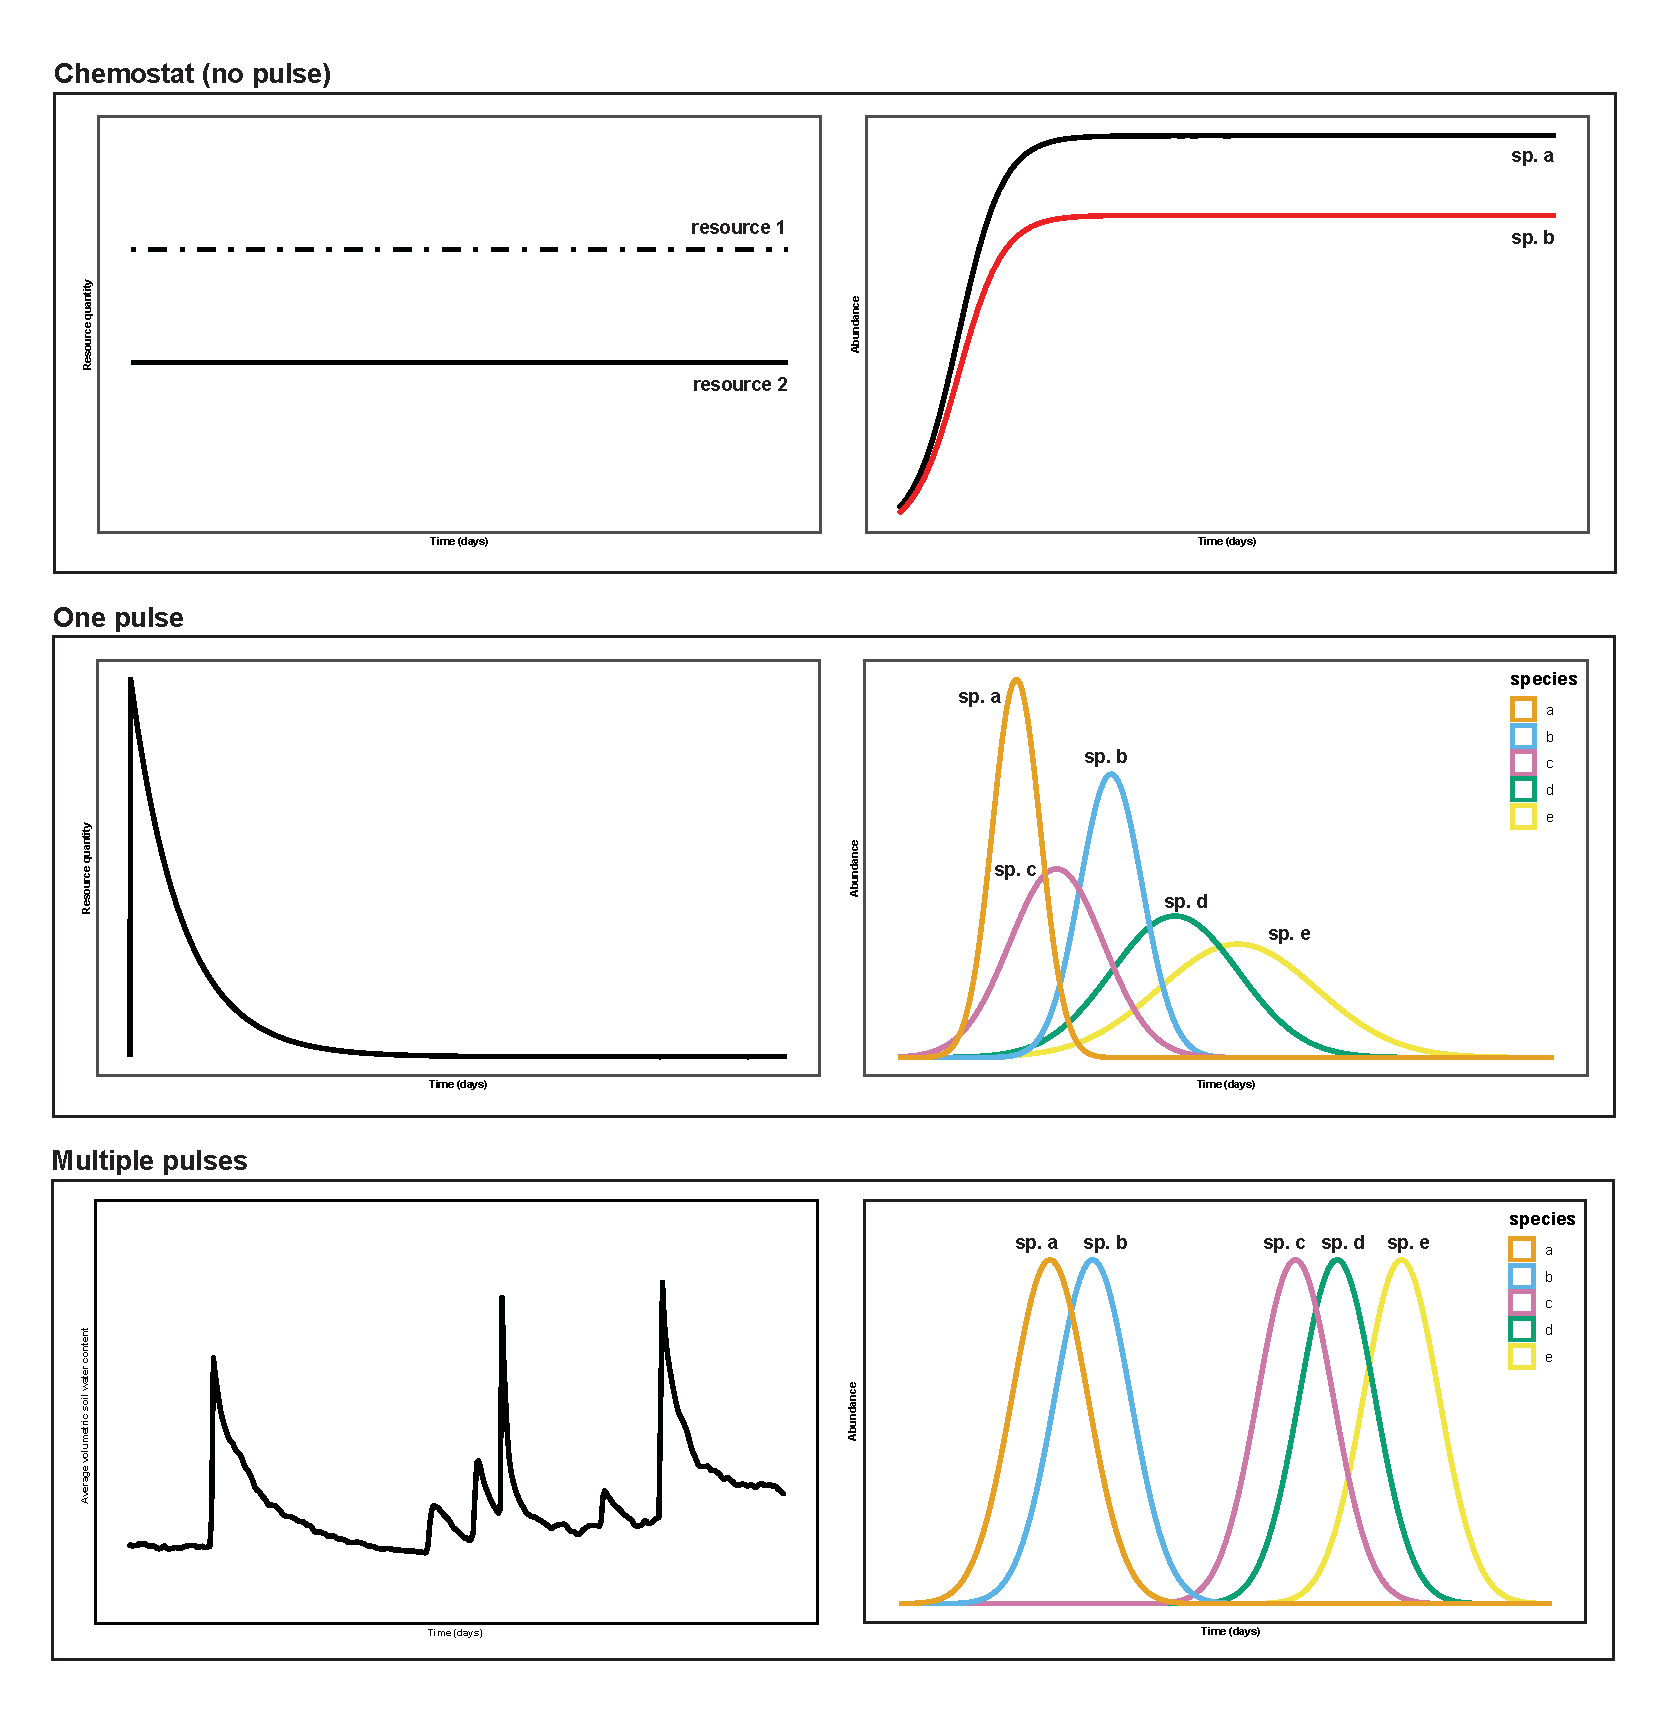
\includegraphics[width=0.8\textwidth]{..//figures/JN_conceptfigs/sixpanel_concept.png}
\caption{Theory suggests resource levels may determine temporal niche space. In a system where resources are constant (top left,, chemostat; species can only coexist if they are each equally good competitors for different resources) species would be expected to show little temporal fluctuations and there would be no real temporal niches. Many models of coexistence today, however, assume a resource pulse that decays (middle, left; e.g., water with evaporative loss, such as in snowpack systems) over time: this resource then sets the temporal window of each season and species compete within it. Most real systems however are more complicated (bottom left, taken from Jornada LTER site 302 showing soil moisture at 10 cm depth over the year) ....} 
% Evaporating single pulse resource: species may invade only at certain levels of resource (includes snowpack/soil nutrients etc.)
%  Multiple pulses: Some species may persist through whole season or use first or second pulse only
 \label{fig:resource}
\end{figure}



\end{document}
